\documentclass[]{report}
\usepackage{graphicx}
\usepackage{float}
\usepackage{amsmath}
\usepackage{amsfonts}
\usepackage{wasysym}

% Title Page
\title{MCEN - 3047}
\author{Jack Goldrick}


\begin{document}
\maketitle

\section{Problem 1}

\subsection{Part A}


	\begin{figure}[H]
	\centering
	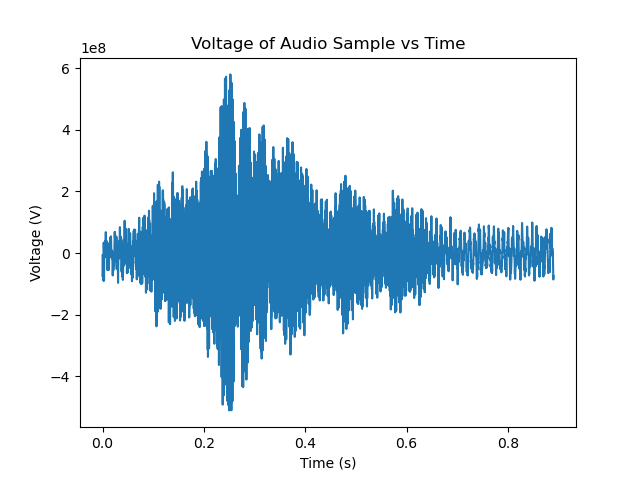
\includegraphics[width=0.7\linewidth]{../results/p1_t}
\end{figure}


\subsection{Part B}

$$ \text{LSB = 8-Bit} $$

\subsection{Part C}

$$V_fs = 709859328.0$$


\section{Problem 2}

\subsection{Part A}

\begin{figure}[H]
	\centering
	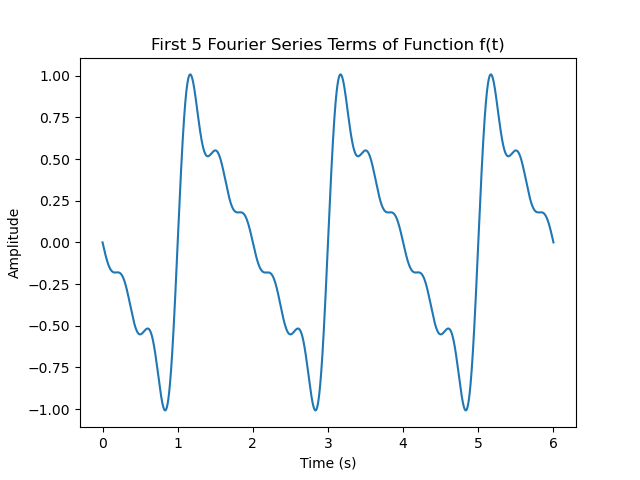
\includegraphics[width=0.7\linewidth]{../results/p2_5}
\end{figure}


\subsection{Part B}


\begin{figure}[H]
	\centering
	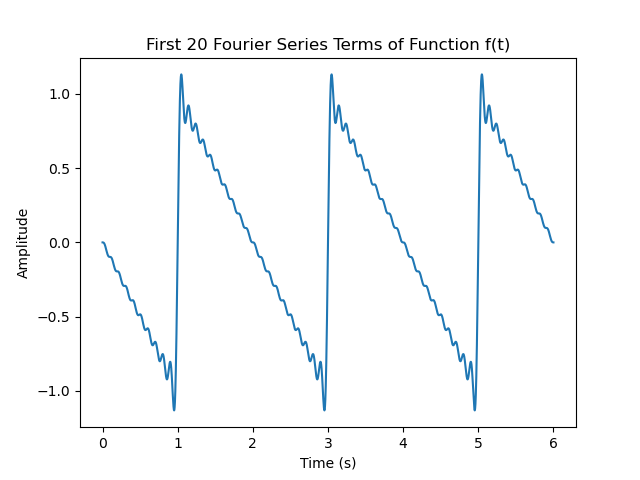
\includegraphics[width=0.7\linewidth]{../results/p2_20}
\end{figure}

\begin{figure}[H]
	\centering
	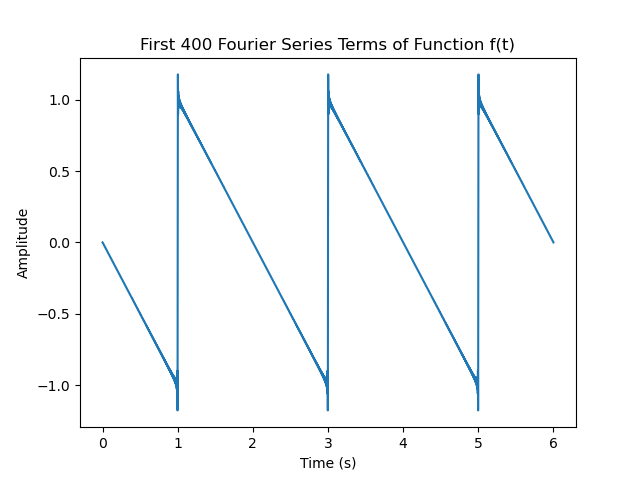
\includegraphics[width=0.7\linewidth]{../results/p2_400}
\end{figure}

\begin{figure}[H]
	\centering
	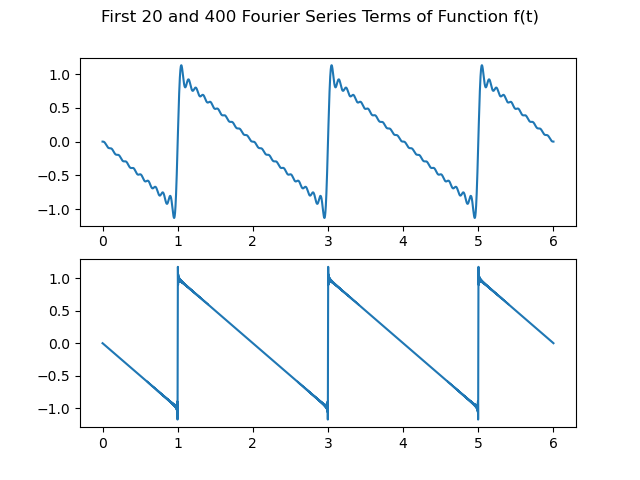
\includegraphics[width=0.7\linewidth]{../results/p2_20_400}
\end{figure}


\subsection{Part C}


\begin{itemize}
	\item The function becomes a better approximation of the cyclical ramp function  as n increases,  The function appears to become more jagged as n increases as well, better approximating digital signals, if it were one. 
\end{itemize}


\section{Problem 3}

\subsection{Part A}

\begin{figure}[H]
	\centering
	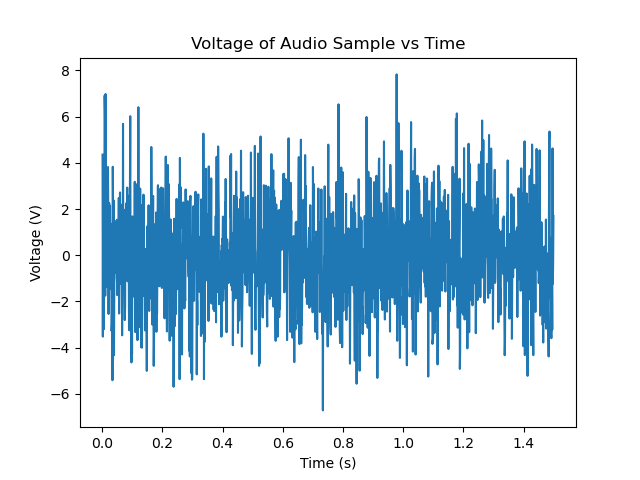
\includegraphics[width=0.7\linewidth]{../results/p3_t}
\end{figure}

\subsection{Part B}

\begin{center}
	It may be possible to get an approximation from this time-series data, however the number may be far from accurate. Thus, one cannot decipher frequency information.
\end{center}

\subsection{Part C}

\begin{figure}[H]
	\centering
	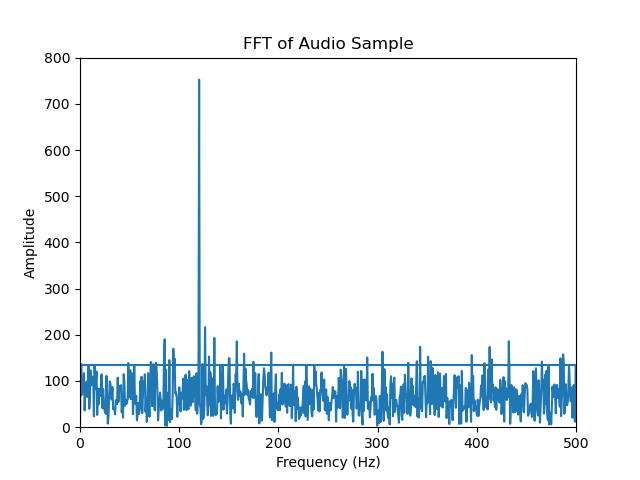
\includegraphics[width=0.7\linewidth]{../results/p3_fft}
\end{figure}


\subsection{Part D}

\begin{center}
	Frequency: 120.0800533689126
\end{center}

\end{document}          




